\documentclass[12pt,a4paper]{article}

% ─── Page Layout ───────────────────────────────────────────────────────────────
\usepackage[a4paper, margin=0.8in, headheight=14pt]{geometry}

% ─── Fonts (XeLaTeX) ───────────────────────────────────────────────────────────
\usepackage{fontspec}
\usepackage{unicode-math}
\setmainfont{TeX Gyre Pagella}
\setmonofont[Scale=0.88]{TeX Gyre Cursor}
\setmathfont{Latin Modern Math}

% ─── Packages ──────────────────────────────────────────────────────────────────
\usepackage{xcolor}
\usepackage{colortbl}
\usepackage{titlesec}
\usepackage{enumitem}
\usepackage{tabularx}
\usepackage{booktabs}
\usepackage{array}
\usepackage{amsmath}
\usepackage{tikz}
\usetikzlibrary{shapes.geometric, arrows.meta, positioning, calc, fit, decorations.pathreplacing, patterns}
\usepackage{tcolorbox}
\tcbuselibrary{skins, breakable}
\usepackage{hyperref}
\usepackage{fancyhdr}
\usepackage{graphicx}
\usepackage{microtype}
\hyphenpenalty=10000
\exhyphenpenalty=10000
\sloppy
\usepackage{caption}
\usepackage{setspace}
\usepackage{multirow}
\usepackage{tocloft}

% ─── Q&A helper ────────────────────────────────────────────────────────────────
\newcommand{\Q}[1]{\textbf{#1}\par\noindent\ignorespaces}

% ─── Colour Palette ────────────────────────────────────────────────────────────
\definecolor{myred}{RGB}{196,30,58}
\definecolor{mydark}{RGB}{30,30,50}
\definecolor{mygreen}{RGB}{14,120,80}
\definecolor{myteal}{RGB}{0,130,140}
\definecolor{myamber}{RGB}{180,100,0}
\definecolor{mypurple}{RGB}{100,30,160}
\definecolor{mygray}{RGB}{246,247,249}
\definecolor{mgframe}{RGB}{180,185,200}
\definecolor{watermark}{RGB}{145,150,170}
\definecolor{hdrred}{RGB}{250,232,235}
\definecolor{hdrgreen}{RGB}{220,244,233}
\definecolor{hdrteal}{RGB}{220,242,244}
\definecolor{hdramber}{RGB}{253,242,215}
\definecolor{hdrpurple}{RGB}{238,228,255}
\definecolor{hdrgray}{RGB}{238,240,245}
\definecolor{rowalt}{RGB}{250,251,253}

% ─── Section Formatting ────────────────────────────────────────────────────────
\titleformat{\section}
  {\large\bfseries\color{myred}}{\thesection.}{0.5em}{}
  [\vspace{1pt}{\color{myred}\rule{\linewidth}{0.8pt}}]
\titleformat{\subsection}
  {\normalsize\bfseries\color{myteal}}{\thesubsection}{0.5em}{}
\titlespacing*{\section}{0pt}{18pt}{7pt}
\titlespacing*{\subsection}{0pt}{11pt}{4pt}

% ─── Paragraph ─────────────────────────────────────────────────────────────────
\setlength{\parindent}{0pt}
\setlength{\parskip}{4pt}

% ─── TOC Styling ───────────────────────────────────────────────────────────────
\renewcommand{\cfttoctitlefont}{\large\bfseries\color{myred}}
\renewcommand{\cftaftertoctitle}{\par\noindent{\color{myred}\rule{\linewidth}{0.8pt}}}
\setlength{\cftbeforetoctitleskip}{0pt}
\setlength{\cftaftertoctitleskip}{6pt}
\renewcommand{\cftsecfont}{\normalsize\bfseries\color{mydark}}
\renewcommand{\cftsecpagefont}{\normalsize\bfseries\color{mydark}}
\renewcommand{\cftsecleader}{\cftdotfill{\cftdotsep}}
\setlength{\cftbeforesecskip}{7pt}
\renewcommand{\cftsubsecfont}{\small\color{mydark}}
\renewcommand{\cftsubsecpagefont}{\small\color{mydark}}
\setlength{\cftbeforesubsecskip}{3pt}
\setlength{\cftsubsecindent}{1.4em}

% ─── Table helpers ─────────────────────────────────────────────────────────────
\renewcommand{\arraystretch}{1.45}
\setlength{\tabcolsep}{6pt}
\arrayrulecolor{mydark}
\newcolumntype{B}[1]{>{\small\bfseries\raggedright\arraybackslash}m{#1}}
\newcolumntype{Y}{>{\small\raggedright\arraybackslash}X}
\renewcommand{\tabularxcolumn}[1]{m{#1}}

% ─── Header / Footer ───────────────────────────────────────────────────────────
\pagestyle{fancy}
\fancyhf{}
\fancyhead[L]{\small\color{myred}\textbf{26-ES-EE101}\;\color{mydark}--- Basic Electrical and Electronics Engineering}
\fancyhead[R]{\small\color{myteal}\textbf{Module 5 Notes}}
\fancyfoot[C]{\small\color{mydark}\thepage}
\fancyfoot[R]{\small\color{watermark}\textit{\copyright\ Biraj}}
\renewcommand{\headrulewidth}{0.5pt}
\renewcommand{\footrulewidth}{0.3pt}

% ─── Hyperref ──────────────────────────────────────────────────────────────────
\hypersetup{
  colorlinks=true, linkcolor=myteal, urlcolor=myteal,
  pdfauthor={Biraj Sarkar (CGEC)},
  pdftitle={26-ES-EE101 --- Module 5 Notes: Semiconductor Fundamentals and Diode Applications}
}

% ─── tcolorbox styles ──────────────────────────────────────────────────────────
\tcbset{
  tikzbox/.style={
    colback=mygray, colframe=mgframe, boxrule=0.6pt, arc=4pt,
    left=8pt, right=8pt, top=6pt, bottom=6pt,
    colbacktitle=mgframe, coltitle=mydark, fonttitle=\small\bfseries
  },
  defbox/.style={
    colback=hdrgreen, colframe=mygreen, boxrule=0.8pt, arc=4pt,
    left=9pt, right=9pt, top=6pt, bottom=6pt,
    colbacktitle=mygreen, coltitle=white, fonttitle=\small\bfseries
  },
  formulabox/.style={
    colback=hdrteal, colframe=myteal, boxrule=0.8pt, arc=4pt,
    left=9pt, right=9pt, top=7pt, bottom=7pt,
    colbacktitle=myteal, coltitle=white, fonttitle=\small\bfseries
  },
  examplebox/.style={
    colback=hdramber, colframe=myamber, boxrule=0.8pt, arc=4pt,
    left=9pt, right=9pt, top=6pt, bottom=6pt,
    colbacktitle=myamber, coltitle=white, fonttitle=\small\bfseries
  },
  masonbox/.style={
    colback=hdrpurple, colframe=mypurple, boxrule=0.8pt, arc=4pt,
    left=9pt, right=9pt, top=6pt, bottom=6pt,
    colbacktitle=mypurple, coltitle=white, fonttitle=\small\bfseries
  },
  exambox/.style={
    colback=hdrpurple, colframe=mypurple, boxrule=1pt, arc=5pt,
    left=10pt, right=10pt, top=8pt, bottom=8pt,
    colbacktitle=mypurple, coltitle=white, fonttitle=\bfseries,
    breakable, title after break={\textbf{Frequently Asked / Viva Questions (contd.)}}
  }
}
\tcbset{breakable}
\tcbset{after={\par\color{black}}}

% ─── TikZ styles ───────────────────────────────────────────────────────────────
\tikzset{
  block/.style={rectangle, draw=myteal, fill=hdrteal,
    text width=2.4cm, align=center, minimum height=0.95cm,
    font=\small, rounded corners=3pt, line width=0.7pt},
  redblock/.style={rectangle, draw=myred, fill=hdrred,
    text width=2.4cm, align=center, minimum height=0.95cm,
    font=\small, rounded corners=3pt, line width=0.7pt},
  sumjunc/.style={circle, draw=myamber, fill=hdramber,
    minimum size=0.62cm, font=\small, line width=0.8pt},
  arrow/.style={-Stealth, thick, color=mydark},
  redarrow/.style={-Stealth, thick, color=myred},
  line/.style={thick, color=mydark}
}

\begin{document}

% ─── Title Page ───────────────────────────────────────────────────────────────
\begin{center}
  {\Large\bfseries\color{myred} 26-ES-EE101}\\[3pt]
  {\LARGE\bfseries\color{myred} Basic Electrical and Electronics Engineering}\\[5pt]
  {\normalsize\color{mydark} Semester I \quad$\bullet$\quad 3L:1T:0P \quad$\bullet$\quad 4 Credits}\\[3pt]
  {\normalsize\color{myteal}\textbf{Module 5 Exam Notes: Semiconductor Fundamentals and Diode Applications}}\\[3pt]
  {\small\color{mydark} CGEC \;$|$\; MAKAUT Syllabus (A.Y. 2026--27) \;$|$\; \textit{Biraj Sarkar}}
\end{center}
\vspace{2pt}
\noindent{\color{myred}\rule{\linewidth}{1.5pt}}
\vspace{2pt}

\hypersetup{linkcolor=mydark}
\tableofcontents
\hypersetup{linkcolor=myteal}
\newpage

\section{Semiconductor Fundamentals and Diode Applications}

\subsection{Energy bands and semiconductor types}
\begin{tcolorbox}[defbox,title={Valence band, conduction band and band gap}]
The valence band contains the states associated with bonding electrons. Electrons in available conduction-band states can move through the solid and contribute to current. The band gap \(E_g\), measured in electronvolts (eV), separates these bands when there are no allowed states between them.
\end{tcolorbox}

\begin{itemize}[leftmargin=*, itemsep=3pt, topsep=4pt]
  \item \textbf{Conductor.} A partly filled band or overlapping bands provide nearby available states.
  \item \textbf{Insulator.} A wide gap leaves few thermally available carriers.
  \item \textbf{Semiconductor.} A smaller gap makes carrier density sensitive to temperature, doping and light.
  \item \textbf{Hole.} A missing electron in a nearly filled valence band behaves as a mobile positive charge.
\end{itemize}

\begin{tcolorbox}[tikzbox,title={Energy-band comparison},unbreakable]
\centering
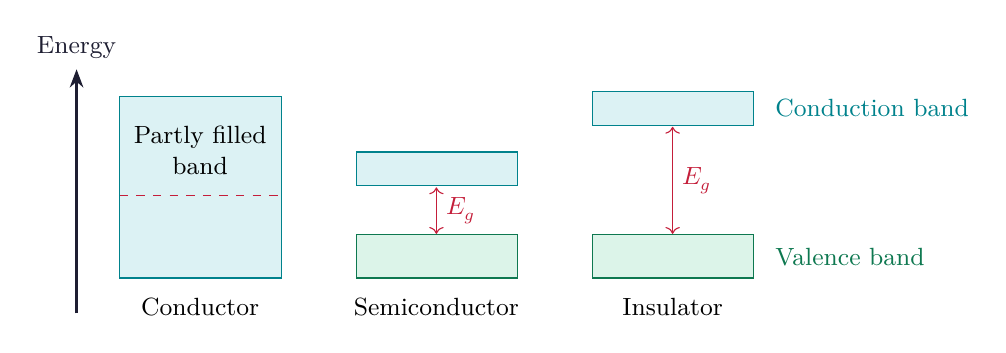
\begin{tikzpicture}[font=\small]
\draw[arrow] (-0.55,0.1)--(-0.55,3.2) node[above] {Energy};
\filldraw[fill=hdrteal,draw=myteal] (0,0.55) rectangle (2.05,2.85);
\draw[myred,dashed] (0,1.60)--(2.05,1.60);
\node[align=center] at (1.02,2.17) {Partly filled\\band};
\foreach \x/\gap in {3.00/0.62,6.00/1.39}{
  \filldraw[fill=hdrgreen,draw=mygreen] (\x,0.55) rectangle ++(2.05,0.55);
  \filldraw[fill=hdrteal,draw=myteal] (\x,{1.10+\gap}) rectangle ++(2.05,0.43);
  \draw[<->,myred] ({\x+1.02},1.11)--({\x+1.02},{1.08+\gap}) node[midway,right] {$E_g$};
}
\node[below] at (1.02,0.42) {Conductor};
\node[below] at (4.02,0.42) {Semiconductor};
\node[below] at (7.02,0.42) {Insulator};
\node[right,myteal] at (8.2,2.71) {Conduction band};
\node[right,mygreen] at (8.2,0.82) {Valence band};
\end{tikzpicture}
\end{tcolorbox}

\begin{itemize}[leftmargin=*, itemsep=3pt, topsep=4pt]
  \item \textbf{Intrinsic.} In undoped material, thermal generation creates electron--hole pairs. At equilibrium \(n=p=n_i\).
  \item \textbf{n-type extrinsic.} Donors such as phosphorus in silicon add available electrons. Electrons are the majority carriers.
  \item \textbf{p-type extrinsic.} Acceptors such as boron in silicon increase the hole concentration. Holes are the majority carriers.
  \item \textbf{Equilibrium check.} Minority carriers remain present and the bulk is electrically neutral. For nondegenerate material at equilibrium, \(np=n_i^2\).
\end{itemize}

\subsection{Drift and diffusion currents}
Drift is carrier motion due to an electric field. Electrons drift against the field and holes drift with the field. Both conventional drift current components point with the field. Diffusion is carrier motion from regions of higher carrier concentration towards lower concentration. In one dimension the conventional current densities are
\[
\begin{aligned}
J_n &= q n\mu_n E+q D_n \frac{dn}{dx},\\
J_p &= q p\mu_p E-q D_p \frac{dp}{dx}.
\end{aligned}
\]
Here \(q>0\) is the elementary charge in C, \(E\) is electric field in V/m, \(n,p\) are in \(\mathrm{m^{-3}}\), \(\mu\) is mobility in \(\mathrm{m^2/(V\,s)}\), \(D\) is diffusivity in \(\mathrm{m^2/s}\), and \(J\) is in \(\mathrm{A/m^2}\). The opposite diffusion signs come from electrons carrying negative charge. For uniform concentration conductivity is \(\sigma=q(n\mu_n+p\mu_p)\), in S/m.

\subsection{The p--n junction and diode characteristic}
\begin{tcolorbox}[defbox,title={Depletion region and bias}]
A p--n junction forms where p-type and n-type regions meet. Near the boundary, majority carriers diffuse and recombine, leaving exposed fixed ions. The resulting region has few mobile carriers and is called the depletion region. Forward bias connects the p-side to higher potential than the n-side. Reverse bias does the opposite.
\end{tcolorbox}

\begin{itemize}[leftmargin=*, itemsep=3pt, topsep=4pt]
  \item \textbf{At equilibrium.} Fixed ions produce a field from n-side to p-side. Diffusion and drift balance.
  \item \textbf{Forward bias.} Lower barrier and narrower depletion region allow strong carrier injection.
  \item \textbf{Reverse bias.} Higher barrier and wider depletion region limit current. Before breakdown the small reverse current is strongly temperature dependent.
\end{itemize}
\[
I_D=I_S\left(e^{V_D/(\eta V_T)}-1\right),\qquad V_T=\frac{kT}{q}\approx25.9\,\mathrm{mV}\quad(300\,\mathrm K).
\]
\begin{itemize}[leftmargin=*, itemsep=3pt, topsep=4pt]
  \item \textbf{Sign convention.} \(V_D\) is anode voltage minus cathode voltage. Positive \(I_D\) flows from anode to cathode. The bar on the circuit symbol marks the cathode.
  \item \textbf{Model parameters.} \(I_S\) is reverse saturation current and \(\eta\) is the ideality factor. Use the exponential model before breakdown, within its applicable current range.
  \item \textbf{Circuit approximation.} For many silicon diode problems, use \(V_D\approx0.7\,\mathrm V\) for a conducting diode at moderate forward current. The forward voltage varies with current and temperature.
\end{itemize}

\begin{tcolorbox}[tikzbox,title={Diode current--voltage characteristic (schematic)},unbreakable]
\centering
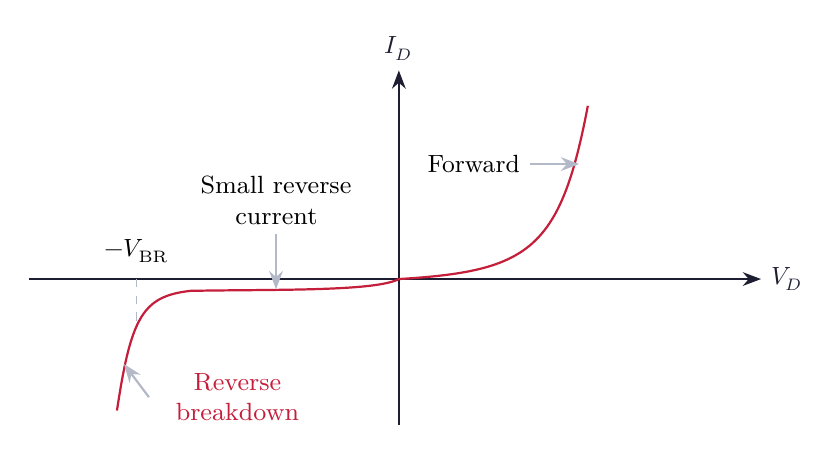
\begin{tikzpicture}[font=\small]
\draw[arrow] (-4.7,0)--(4.6,0) node[right] {$V_D$};
\draw[arrow] (0,-1.85)--(0,2.65) node[above] {$I_D$};
\draw[myred,thick] (-3.58,-1.67) .. controls (-3.40,-0.47) and (-3.25,-0.22) .. (-2.65,-0.15)
  .. controls (-1.6,-0.13) and (-0.3,-0.16) .. (0,0)
  .. controls (1.65,0.1) and (2.05,0.36) .. (2.4,2.2);
\draw[dashed,mgframe] (-3.33,0)--(-3.33,-0.59);
\node[above] at (-3.33,0.08) {$-V_{\mathrm{BR}}$};
\node[myred,align=center,text width=2cm] (breakdown) at (-2.05,-1.50) {Reverse\\breakdown};
\draw[arrow,mgframe] (breakdown.west)--(-3.49,-1.08);
\node (forward) at (0.95,1.46) {Forward};
\draw[arrow,mgframe] (forward.east)--(2.29,1.46);
\node[align=center,text width=2.5cm] (leakage) at (-1.56,1.00) {Small reverse\\current};
\draw[arrow,mgframe] (leakage.south)--(-1.56,-0.13);
\end{tikzpicture}
\end{tcolorbox}

\begin{itemize}[leftmargin=*, itemsep=3pt, topsep=4pt]
  \item \textbf{Zener breakdown.} Tunnelling through the narrow depletion region of a heavily doped junction.
  \item \textbf{Avalanche breakdown.} Impact ionisation creates more electron--hole pairs. It is favoured by a wider depletion region and generally higher breakdown voltage.
  \item \textbf{Practical point.} The mechanisms can coexist. Limit current to the device rating when using breakdown.
\end{itemize}

\subsection{Half-wave and full-wave rectifiers}
A \textbf{rectifier} converts an AC input into a unidirectional output. For a resistive load and ideal diodes:
\begin{itemize}[leftmargin=*, itemsep=3pt, topsep=4pt]
  \item \textbf{Half-wave.} One series diode conducts in one half cycle.
  \item \textbf{Centre-tapped full-wave.} Two diodes use alternate half-secondary windings. Load current has the same direction in both halves.
  \item \textbf{Bridge full-wave.} Four diodes use the full secondary. Two conduct per half cycle with the same load-current direction. Opposite corners receive AC. The common cathodes give the positive output and the common anodes the negative output.
\end{itemize}

\begin{tcolorbox}[tikzbox,title={Bridge rectifier and conducting paths},unbreakable]
\centering
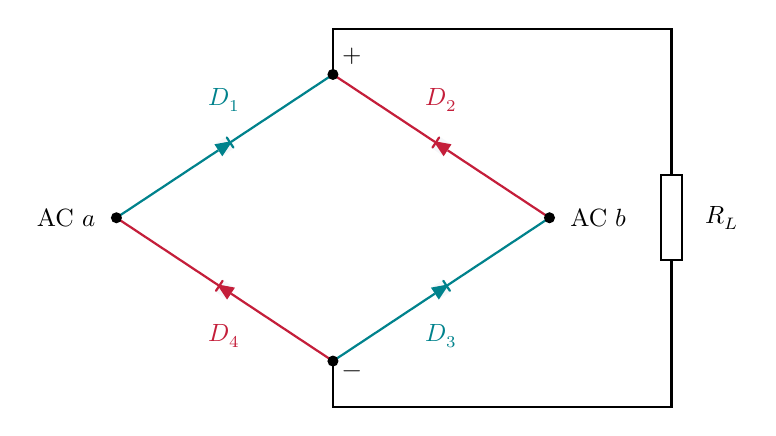
\begin{tikzpicture}[font=\small,line cap=round]
\coordinate (A) at (-2.75,0);
\coordinate (B) at (2.75,0);
\coordinate (P) at (0,1.82);
\coordinate (N) at (0,-1.82);
\foreach \from/\to/\lab/\clr/\side in {A/P/$D_1$/myteal/above,B/P/$D_2$/myred/above,N/B/$D_3$/myteal/below,N/A/$D_4$/myred/below}{
  \draw[thick,\clr] (\from)--(\to);
  \path (\from)--(\to) node[midway,sloped,allow upside down,fill=mygray,inner sep=0pt] {
    \tikz[baseline=-0.5ex,x=1em,y=1em]{
      \filldraw[fill=mygray,thick,\clr] (-0.32,-0.22)--(-0.32,0.22)--(0.20,0)--cycle;
      \draw[thick,\clr] (0.20,-0.24)--(0.20,0.24);
    }};
  \path (\from)--(\to) node[midway,\side=9pt,text=\clr] {\lab};
}
\draw[thick] (P)--(0,2.40)--(4.3,2.40)--(4.3,0.54)
  (4.3,-0.54)--(4.3,-2.40)--(0,-2.40)--(N);
\draw[thick,fill=white] (4.17,-0.54) rectangle (4.43,0.54);
\node[right=5pt] at (4.43,0) {$R_L$};
\fill (A) circle (2pt) (B) circle (2pt) (P) circle (2pt) (N) circle (2pt);
\node[left=4pt] at (A) {AC $a$};
\node[right=4pt] at (B) {AC $b$};
\node[above right] at (P) {$+$};
\node[below right] at (N) {$-$};
\end{tikzpicture}
\par\smallskip\small
\(a\) positive relative to \(b\): \(D_1,D_3\) conduct.
\quad \(b\) positive relative to \(a\): \(D_2,D_4\) conduct.
\end{tcolorbox}

\begin{tcolorbox}[tikzbox,title={Ideal unfiltered output waveforms},unbreakable]
\centering
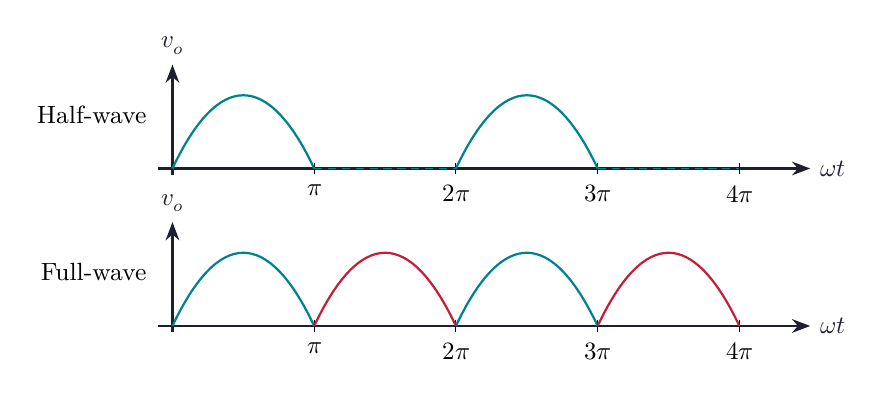
\begin{tikzpicture}[x=0.90cm,y=0.80cm,font=\small]
\foreach \y/\name in {2.5/Half-wave,0/Full-wave}{
  \node[left] at (-0.23,{\y+0.85}) {\name};
  \draw[arrow] (-0.2,\y)--(9.0,\y) node[right] {$\omega t$};
  \draw[arrow] (0,{\y-0.10})--(0,{\y+1.65}) node[above] {$v_o$};
  \foreach \x/\lab in {2/{\pi},4/{2\pi},6/{3\pi},8/{4\pi}}{
    \draw (\x,{\y-0.09})--(\x,{\y+0.09});
    \node[below] at (\x,{\y-0.11}) {$\lab$};
  }
  \foreach \x in {0,4}{
    \draw[myteal,thick] (\x,\y) .. controls ({\x+0.65},{\y+1.55})
    and ({\x+1.35},{\y+1.55}) .. ({\x+2},\y);
  }
}
\draw[myteal,thin,densely dashed] (2,2.5)--(4,2.5) (6,2.5)--(8,2.5);
\foreach \x in {2,6}{
  \draw[myred,thick] (\x,0) .. controls ({\x+0.65},1.55)
    and ({\x+1.35},1.55) .. ({\x+2},0);
}
\end{tikzpicture}
\end{tcolorbox}

For input frequency \(f\) and a peak output pulse \(V_m\) in the ideal unfiltered circuit,
\[
\begin{aligned}
V_{\mathrm{DC,half}}
 &=\frac{1}{2\pi}\int_0^\pi V_m\sin\theta\,d\theta
 =\frac{V_m}{\pi},\\
V_{\mathrm{DC,full}}
 &=\frac{2}{2\pi}\int_0^\pi V_m\sin\theta\,d\theta
 =\frac{2V_m}{\pi}.
\end{aligned}
\]
Supply the appropriate \(V_m\): in a centre-tapped design it is the peak of one half-secondary, and in a bridge it is the full-secondary peak. For the unfiltered ideal circuit the peak inverse voltage (PIV) per diode is \(V_m\) in half-wave and bridge circuits and \(2V_m\) in the centre-tapped circuit. A reservoir capacitor changes the off-state voltage in some topologies. With a real bridge take off approximately two forward drops from the peak.

\subsection{Filters and Zener voltage regulation}
A \textbf{filter} reduces AC ripple after rectification. A shunt capacitor charges near the peaks and supplies the load between them. For small ripple, approximate the discharge by \(\Delta Q=I_L/f_{\mathrm{ripple}}\). Since \(\Delta Q=C\Delta V\),
\[
\Delta V_{\mathrm{pp}}\approx\frac{I_L}{f_{\mathrm{ripple}}C},
\]
with \(f_{\mathrm{ripple}}=f\) for half-wave and \(2f\) for full-wave. The average filtered voltage is roughly the charged peak minus half the peak-to-peak ripple. An LC filter uses a series inductor to oppose ripple current and a shunt capacitor to bypass it. A capacitor--inductor--capacitor arrangement is called a \(\pi\) filter.

\begin{tcolorbox}[examplebox,title={Estimate the output from a filtered bridge}]
A \(12\,\mathrm{V}\) RMS, \(50\,\mathrm{Hz}\) secondary feeds a bridge with \(0.7\,\mathrm V\) per forward diode, \(C=1000\,\mu\mathrm F\) and \(I_L=0.10\,\mathrm A\).
\[
\begin{aligned}
V_{\mathrm{peak}}&\approx 12\sqrt2-2(0.7)=15.57\,\mathrm V,\\
\Delta V_{\mathrm{pp}}&\approx\frac{0.10}{100(1000\times10^{-6})}=1.00\,\mathrm V,\\
V_{\mathrm{DC}}&\approx15.57-\frac{1.00}{2}=15.07\,\mathrm V .
\end{aligned}
\]
\end{tcolorbox}

In a \textbf{Zener shunt regulator}, a series resistor \(R_S\) connects \(V_{\mathrm{in}}\) to the output. The reverse-biased Zener and load are in parallel, with the Zener cathode at the positive output. In breakdown \(V_o\approx V_Z\), and
\[
\begin{aligned}
I_S&=\frac{V_{\mathrm{in}}-V_Z}{R_S},\\
I_Z&=I_S-I_L,\qquad P_Z\approx V_Z I_Z .
\end{aligned}
\]
\begin{itemize}[leftmargin=*, itemsep=3pt, topsep=4pt]
  \item \textbf{Minimum current check.} Use minimum input voltage and maximum load current.
  \item \textbf{Maximum dissipation check.} Use maximum input voltage and minimum load current.
\end{itemize}
\begin{tcolorbox}[examplebox,title={Shunt-regulator current and power}]
For \(V_{\mathrm{in}}=12\,\mathrm V\), \(V_Z=5.1\,\mathrm V\), \(R_S=330\,\Omega\) and \(I_L=10\,\mathrm{mA}\),
\[
\begin{aligned}
I_S &= (12-5.1)/330 \approx20.91\,\mathrm{mA},\\
I_Z &= I_S-I_L \approx10.91\,\mathrm{mA},\\
P_Z &= V_Z I_Z \approx55.6\,\mathrm{mW}.
\end{aligned}
\]
\end{tcolorbox}

\subsection{Light-emitting diode and photodiode}
\begin{itemize}[leftmargin=*, itemsep=3pt, topsep=4pt]
  \item \textbf{Light-emitting diode (LED).} Forward-bias recombination emits photons. The material influences their energy \(hf\) and wavelength. Symbol arrows point outwards.
  \item \textbf{Current limiting.} Use a series resistor. For a \(5\,\mathrm V\) supply, a \(2\,\mathrm V\) LED and target \(10\,\mathrm{mA}\), \(R=(5-2)/0.01=300\,\Omega\).
  \item \textbf{Photodiode.} Incoming photons generate carriers. The depletion field separates them and gives a photocurrent proportional to light power in the linear region. Symbol arrows point inwards.
  \item \textbf{Bias and applications.} A photodiode can operate at zero bias or in reverse bias for a faster response. Dark current is the reverse current without light. Uses include optical links, light meters and sensors.
\end{itemize}



\newpage
\begin{center}
  {\large\bfseries\color{myred} Quick Revision --- Module 5}\\[3pt]
  {\small\color{mydark} Semiconductor Fundamentals and Diode Applications $|$ 26-ES-EE101}
\end{center}
\noindent{\color{myred}\rule{\linewidth}{1.2pt}}
\vspace{4pt}

\begin{tcolorbox}[formulabox, title={Key Formulas and Concepts at a Glance}]
\renewcommand{\arraystretch}{1.35}
\begin{tabularx}{\linewidth}{B{4.4cm}Y}
Thermal equilibrium & $np=n_i^2$; in intrinsic material $n=p=n_i$. \\[3pt]
Diode equation & $I_D=I_S[\exp(V_D/(\eta V_T))-1]$ before breakdown. \\[3pt]
Ideal mean rectifier output & $V_m/\pi$ for half-wave; $2V_m/\pi$ for full-wave. \\[3pt]
Capacitor ripple & $\Delta V_{\mathrm{pp}}\approx I_L/(f_{\mathrm{ripple}}C)$. \\[3pt]
Shunt regulation & $I_Z=(V_{\mathrm{in}}-V_Z)/R_S-I_L$. \\[3pt]
\end{tabularx}
\end{tcolorbox}

\begin{tcolorbox}[defbox, title={One-Line Definitions}]
\textbf{Band gap.} Energy interval without allowed states between the valence and conduction bands.

\textbf{Depletion region.} Junction region depleted of mobile carriers and containing exposed fixed ions.

\textbf{Ripple.} AC variation remaining on a rectified DC output.
\end{tcolorbox}

\begin{tcolorbox}[exambox, title={Frequently Asked / Viva Questions}]
\begin{enumerate}[topsep=0pt, label=\textbf{Q\arabic*.}, itemsep=5pt]
  \item \Q{What is a hole?} A missing valence-band electron that acts as a positive mobile carrier.
  \item \Q{What does a donor add?} A donor adds an available electron, increasing the electron concentration.
  \item \Q{How do drift and diffusion differ?} Drift is field-driven. Diffusion is driven by concentration gradients.
  \item \Q{What happens to the barrier in forward bias?} The applied voltage reduces the barrier and narrows the depletion region.
  \item \Q{What distinguishes Zener and avalanche breakdown?} Tunnelling versus impact ionisation.
  \item \Q{Why is a bridge full wave?} A different diode pair conducts each half cycle, maintaining the load-current direction.
  \item \Q{How does a reservoir capacitor reduce ripple?} It supplies load current between successive peaks.
  \item \Q{Which conditions give the largest Zener current?} Highest input voltage and lightest load, while the diode regulates.
  \item \Q{Why use an LED series resistor?} It limits current to the intended operating value.
  \item \Q{What is a photodiode's dark current?} Reverse current measured without optical illumination.
\end{enumerate}
\end{tcolorbox}

\begin{tcolorbox}[tikzbox, title={Summary Reference}]
\begin{tabularx}{\linewidth}{|B{4.0cm}|Y|}\hline
Topic & \textbf{What to remember} \\ \hline
Unfiltered half-wave & One pulse per supply cycle. \\ \hline
Unfiltered full-wave & Two pulses per supply cycle. \\ \hline
Filter and regulator & The filter reduces ripple. The regulator stabilises the output voltage. \\ \hline
LED and photodiode & The LED emits light. The photodiode senses it. \\ \hline
\end{tabularx}
\end{tcolorbox}

\end{document}

